\chapter{Managing Object Lifetime}
%Every object created by your application lives for an interval of time from its
%creation to the point that the Java runtime gets around to collecting it. An object's {\em natural} lifetime is defined by the
%interval of time between its first and last necessary use. %cite drag paper
%here?

In a \emph{well-behaved} application, an object's lifetime spans its allocation,
use, and the short period during which the \jre takes control and reclaims the
space. For some subset of an object's actual lifetime, that is the time from
creation to reclamation, your application will make use of the data stored in its
fields. \autoref{fig:typical-lifecycle} illustrates the lifecycle of a typical
object in a well behaved application.

\begin{figure}
	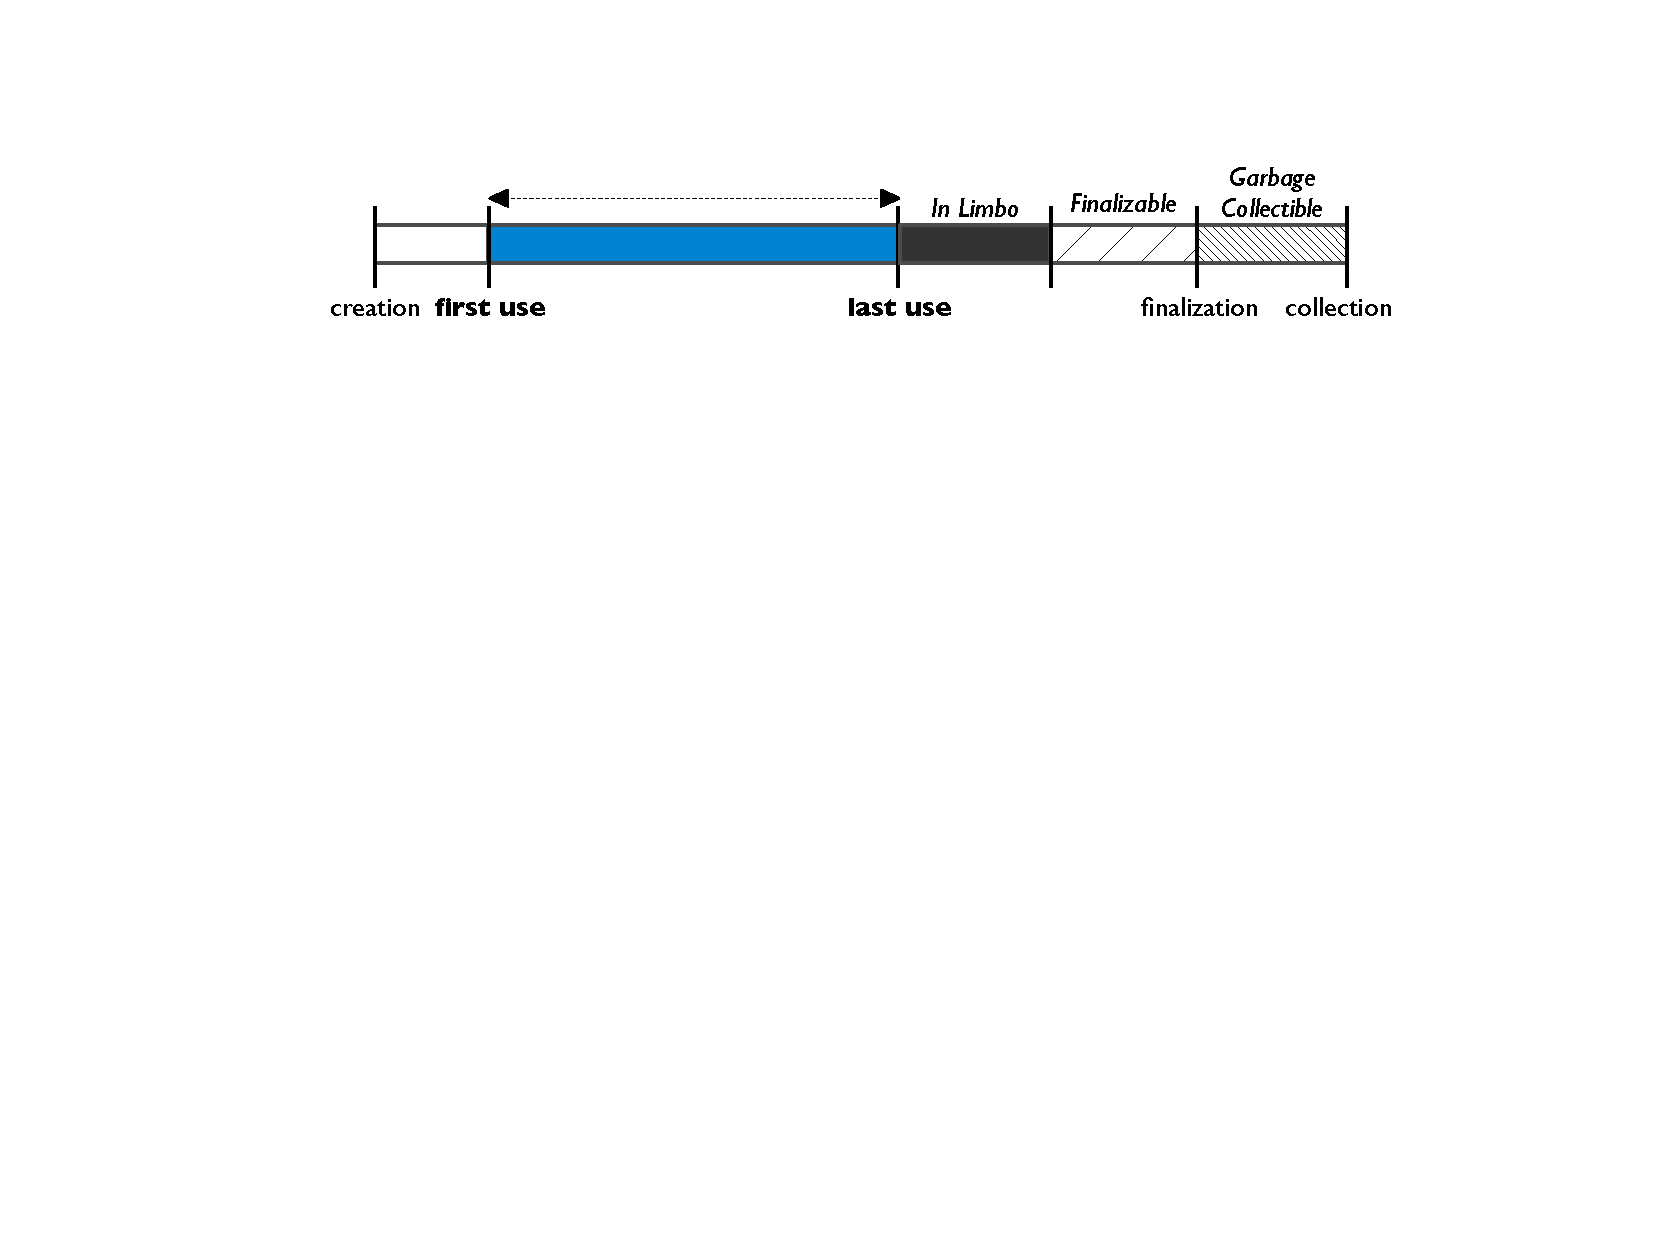
\includegraphics[width=0.9\textwidth]{Figures/lifetime/object-lifecycle}
	\caption{Timeline of the life of an object.}
	\label{fig:typical-lifecycle}
\end{figure}

\begin{example}{Parsing a Date} Consider a loop that shows an easy way to parse
a list of dates. What objects are created, and what are their lifetimes?
\begin{shortlisting}
for (String string : inputList) {
	ParsePosition pos = new ParsePosition(0);
	SimpleDateFormat parser = new SimpleDateFormat();
	System.out.println(parser.parse(string, pos));
}
\end{shortlisting}
\end{example}

For each iteration of this loop, this code takes a date that is represented as a
string and produces a standard Java \class{Date} object. In doing so, a number of
objects are created. Two of these are easy to see, in the two \code{new} calls
that create the parse position and date parser objects. The programmer who wrote
this created two objects, but many more are created by the standard libraries to
finish the task. These include a calendar object, number of arrays, and the
\class{Date} itself. None of these objects are used beyond the iteration of the
loop in which they were created. Within one iteration, they are created, almost
immediately used, and then enter a state of \emph{limbo}.

\callout{limbo}{Objects in Limbo}{
\index{Limbo}
In limbo, an object will never be used again, or at least not for long time,
but the \jre doesn't yet know that this is the case. The object hangs
around, taking up space in the Java heap until the point when it exits limbo.}

The \code{pos} object represents to the parser the position within the
input string to begin parsing. The implementation of the \code{parse} method
uses it early on in the process of parsing. Despite being unused for the
remainder of the parsing, the \jre does not know this until the current
iteration of the loop has finished. This time in limbo also includes the
entirety of the call to \code{System.out.println}, an operation entirely
unrelated to the creation or use of the parse position object. Once the current
loop iteration finishes, these two objects will exit limbo, and become garbage
collectible.\index{Exiting Limbo}

\begin{figure}
	\centering
	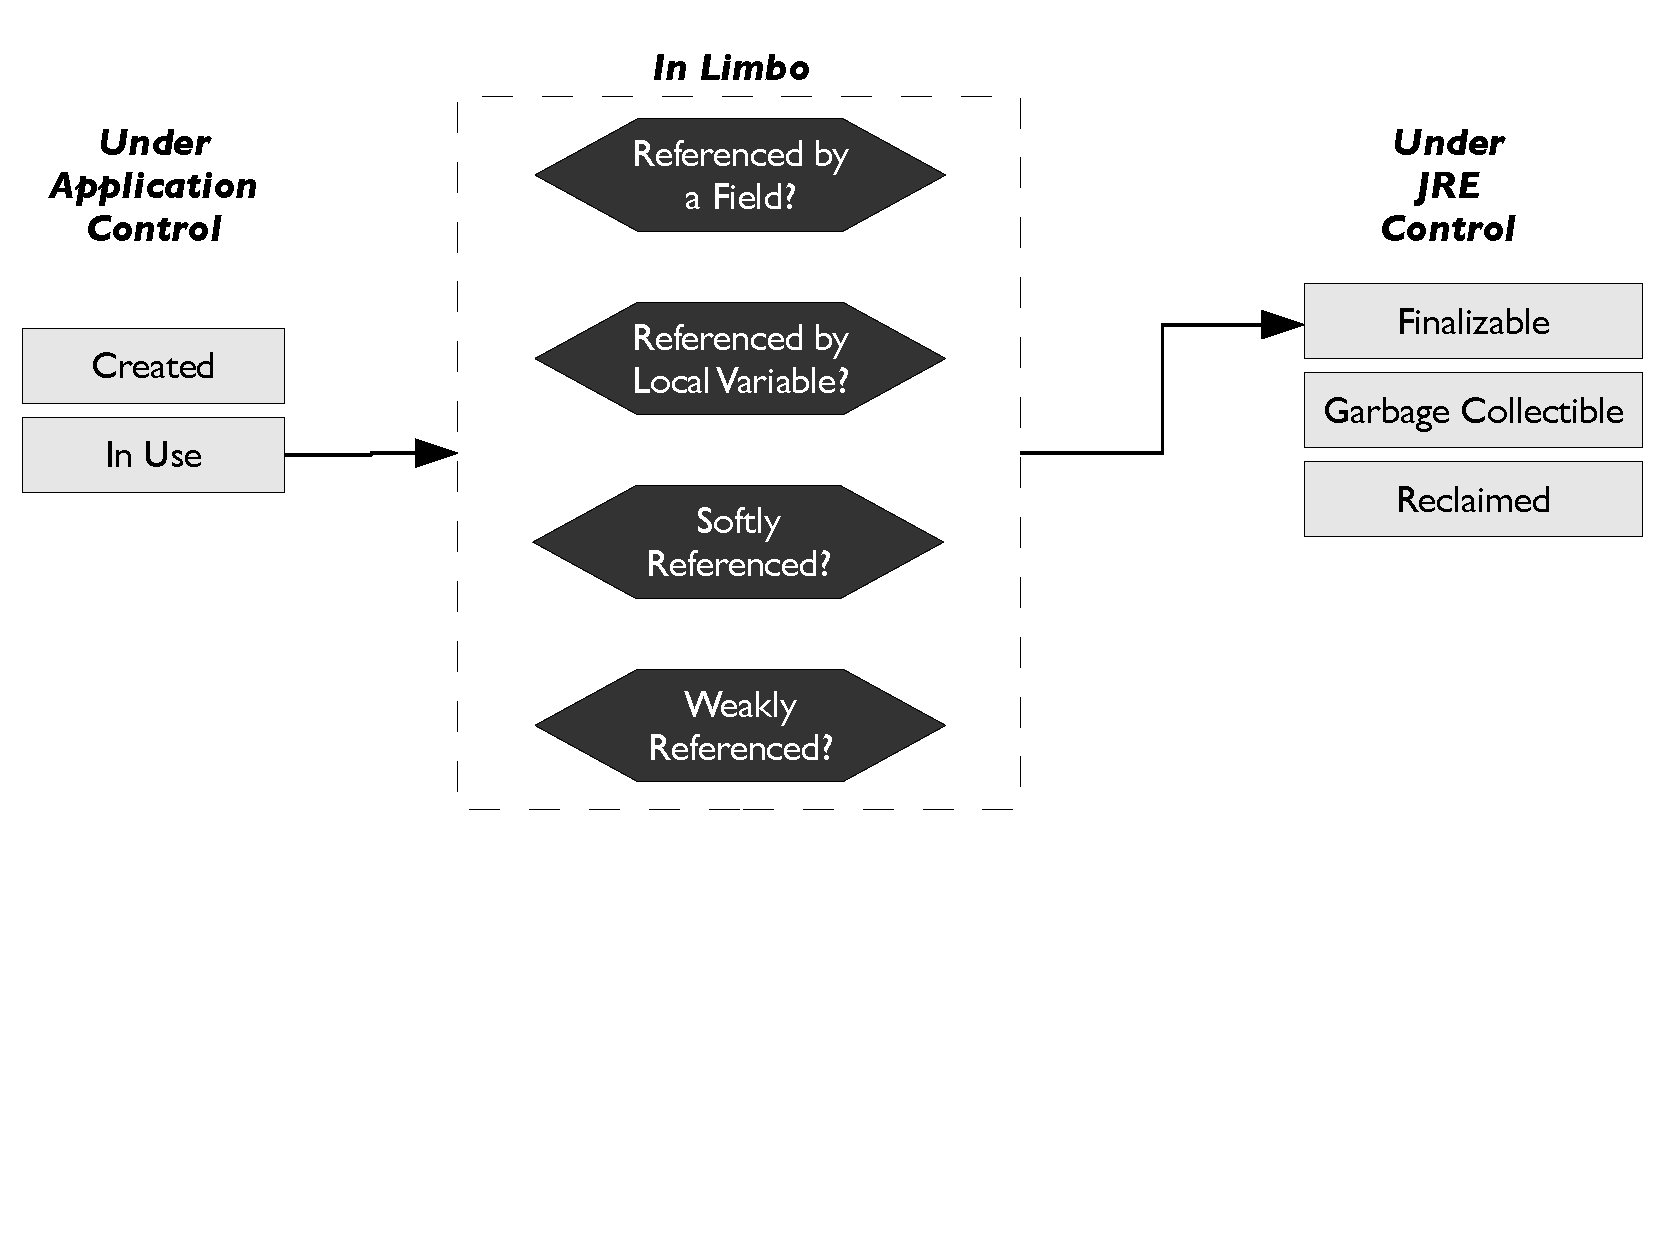
\includegraphics[width=\textwidth]{Figures/lifetime/states}
	\caption{After its last use, an object enters a kind of limbo: the application
	is done with it, but the \jre hasn't yet inferred this to be the case. When an
	object exits limbo depends on the way it is referenced.}
		\label{fig:limbo-exit}
\end{figure}

\section{Basic Management Mechanisms}

The point at which an object exits its limbo depends upon how it is referenced by
other objects. One can always assure that an object exits limbo by modifying your
code to overwrite all references to that variable. If an object is no longer
referenced at all, then it will exit limbo immediately.\footnote{Talk about
reference cycles?} For example, a common way to do this is by assigning
references to the value \code{null}. This is tricky in many cases, because it may not be easy to
know where all those references emanate from. Who is to say that, when one calls
the \code{parse} method of a \class{SimpleDateFormat} object, that it does not
squirrel away a reference to the \class{ParsePosition} passed as a parameter? The
API contract for \code{parse} makes no such claims, one way or the other. This is
certainly calls to mind the worst of the days of explicitly managing memory in a
language like C.


\begin{table}
\centering
	\begin{tabular}{ll} \toprule reachable only from  & moment
	when object exits limbo \\ \cmidrule(r){1-1} \cmidrule(l){2-2}
			%
			nothing & immediately
        	\\
        	%
        	local variable & after scope exits
        	\\ \addlinespace
        	%
        	instance field of an object & 
        	when that object exits limbo %(could be \emph{never} --- memory leak)
        	\\
        	%
        	static field of an object &
        	when that object's class is unloaded
        	%
        	\\ \addlinespace
        	field of \class{WeakReference} & immediately
        	\\
        	%
        	field of \class{SoftReference} & approximately
        	LRU%$^{**}$
        	%
        	\\
        	$\ldots$ with \class{ReferenceQueue} & $\ldots$ then, after removed
        	from queue
        	%
        	\\ \addlinespace
        	entry in thread local storage & when that thread dies
        	%
        	\\ 
        \bottomrule
    \end{tabular}
	\caption{When, or
	even whether, an object exits limbo depends upon how your program references
	it. If these references aren't explicitly overwritten, e.g. by your
	code expliclty assigning the reference to \code{null}, then an object only
	exits limbo under certain restricted circumstances.
%	The point when an object exits limbo depends on 
	%decisions under programmer control: it depends on how the object is
	%referenced.
	%older {\jre}s	use very poor heuristics for handling soft references; see the
	% body for more detail.
	%, it will be reclaimed
	%under certain rules, or may be part of a memory leak
	}
	\label{tab:limbo-exit}
\end{table}

Still, one can't always rely on automatic mechanisms to guide an object out of
limbo in a timely fashion.
\autoref{fig:limbo-exit} and \autoref{tab:limbo-exit}
illustrate how an object may exit limbo. 
A garbage collector only knows that an object is ready to
be collected based on {\em reachability}: how the objects point to eachother.
If, as in the \class{ParsePosition}
or \class{SimpleDateFormat} objects from our example, the object is referenced
only by a local variable of a method, the \jre will not consider reclaming its
storage until the variable's scope exits; e.g. when the loop continues to the
next iteration, or when the method returns, depending on the scope of the
variable that references the object. If the object is referenced only by a
field of another object, then it must wait for that other object to exit limbo
before it can do so. 
An objects pointed to be only by a static field has a good chance of never
being collected. A class only exits limbo when it is unloaded by the \jres
class loading mechanism, which is unlikely to happen if it has static fields
that reference other objects. Therefore, unless that field is overwritten,
objects pointed to by static fields are likely never to exit limbo.

\section{More Complex Management Mechanisms}
There are important lifetime management policies that are not expressible via the
normal mechanisms. When referenced by a local variable, an object lives or dies
with the scope of the variable; when referenced by another object, it lives or
dies along with that object (both, of course, in the absence of overwriting a
reference). The Java specification provides three other mechanisms that let you
guide the \jre to the right time for an object to exit limbo: weak references,
soft references, and thread-local storage.

\subsection{Weak References}
\index{Weak Reference}

Java provides a low-level mechanism that one can use to implement a
correlated lifetime memory management policy, in the form of weak references.
The standard library exposes this feature in the class
\class{java.util.WeakReference}. Using this class correctly is
difficult, because the semantics of weak references does not directly map to
any important application-level use cases.

\begin{definition}
When calling the constructor \class{new WeakReference(obj)},
 this new instance will maintain a reference to \code{obj}, however
 \code{obj} will exit limbo, and become a candidate for cleanup processing by 
the \jre, as if that reference did not exist.
\end{definition} 

When used in this way, weak references don't keep an object alive longer than it
otherwise would have, in the absence of weak references. 
This seems pretty far from anything an application might
need. Still, you can use this low-level feature to implemented correlated
lifetime, as long as you're careful. 
When used to implement correlated lifetime policies, weak references may
indeed delay the time till an object exits limbo.
Improper use of a \class{WeakReference} will
render your code worse off than before. It is quite possible that you will not
have achieved the correlated lifetime that you need, but in a way that is hard
to tell. Even worse, when using weak references, you can introduce memory
leaks. Be very cautious when using them, and follow these rules.

\callout{weaks}{Rules for Using \class{java.util.WeakReference}}{
	In order to assure that you use of weak references works properly, you must
	follow three rules:
	\begin{itemize}
      \item Your instances of \class{WeakReference} must not, directly or
      indirectly, maintain a non-weak reference to the object you wish to
      annotate. It is best to maintain a collection of non-weak references to
      the annotated objects, and use a local variable, or a subclass of
      \class{WeakReference} for any other ways you refer to the annotated object.
      
      \item You must ensure that the \class{WeakReference} objects (or
      subclasses thereof) that you create will exit limbo no sooner than the
      annotated objects. Otherwise, these objects themselves, following the
      rules of \autoref{tab:limbo-exit}, will exit limbo too early. So, if the
      annotated objects are referenced by a collection that is in turn
      referenced by a static field, then the same must be true for the weak
      reference objects as well. 

      \item Since you have to maintain two, parallel, collections to maintain
      references to the annotated objects, and to the annotations, you must
      ensure that exit limbo in lockstep. It is best to create your instances
      of \class{WeakReference} with a \class{ReferenceQueue} parameter. You
      must periodically call \code{poll} on this queue, and remove the
      \class{WeakReference} instances from the parallel registry.
    \end{itemize}
}

You can see that, despite the benefit of some support from the \jre, there
is quite a bit of memory management that you are left with. Luckly, the
standard library ships with a \class{WeakHashMap}\index{WeakHashMap} which deals
with some, but not all, of the legwork of managing weak references. It will
handle the second and third items, but not the first. It is still up to you to
ensure that none of your annotations, directly or indirectly, reference the
annotated object. 

\begin{example}{Timestamp Annotation}
How can you associate a timestamp with an object in a way that avoids memory
leaks and that scales well to a highly concurrent workload?
\end{example}

We can start with the following code:

\begin{shortlisting}
class TimestampAnnotation<T> {
	T t;
	long timestamp;
}
List annotations;
for (String string : inputList) {
	...
	annotations.add(new WeakReference(new Wrapper<String>(string)));
	...
}
\end{shortlisting}

Despite your use of \class{WeakReference}, you would find that neither the main
object (the strings), nor the annotations, would ever be collected. This code
has two memory leaks. One of the leaks is due to a
violation of the first principal of the use of weak references: the annotations
strongly reference the objects being annotated. It is not always this easy to
debug problems in using weak references. Your application will hold on to objects
that you didn't expect. Quite often, it is difficult to even know that there is a
problem in the first place! The application may behave normally, except that it
will consume more memory than necessary; if this extra memory consumption pushes
it over your maximum heap size, then your application will crash --- you will
know something is wrong, but diagnosing this type of problem, a memory
leak\index{Memory Leak}, is quite difficult. It is better to keep the
three principles of weak references in mind, and design in a way that avoids
memory leaks in the first place. Your annotations can be modified to use a
\class{WeakReference} to the main object:

\begin{shortlisting}
class TimestampAnnotation<T> {
	WeakReference<T> t; // annotation only weakly refs main object
	long timestamp;
	
	TimestampAnnotation(T t) {
		this.t = new WeakReference(t);
	}
}
\end{shortlisting}

In this case, the annotation has no normal references to the annotated object,
and so it obides by the first rule of weak references. If you remember from
\autoref{chapter:delegation}, the code can be improved further to avoid the cost
of delegation. This version of the annotation class extends
\class{WeakReference}:

\begin{shortlisting}
class TimestampAnnotation<T> extends WeakReference<T> {
	long timestamp;
	
	TimestampAnnotation(T t) {
		super(t);
	}
}
\end{shortlisting}

Unfortunately, both of these updated versions h

\subsection{Soft References}
\index{Soft Reference}

\subsection{Properly Draining a Reference Queue}

\subsection{Thread-local Storage}
\index{Thread-local Storage}


\begin{comment}
\begin{figure}
	\centering
	\subfigure[The lifecycle of a typical object and its data.]{
	\label{fig:typical-lifecycle1}
			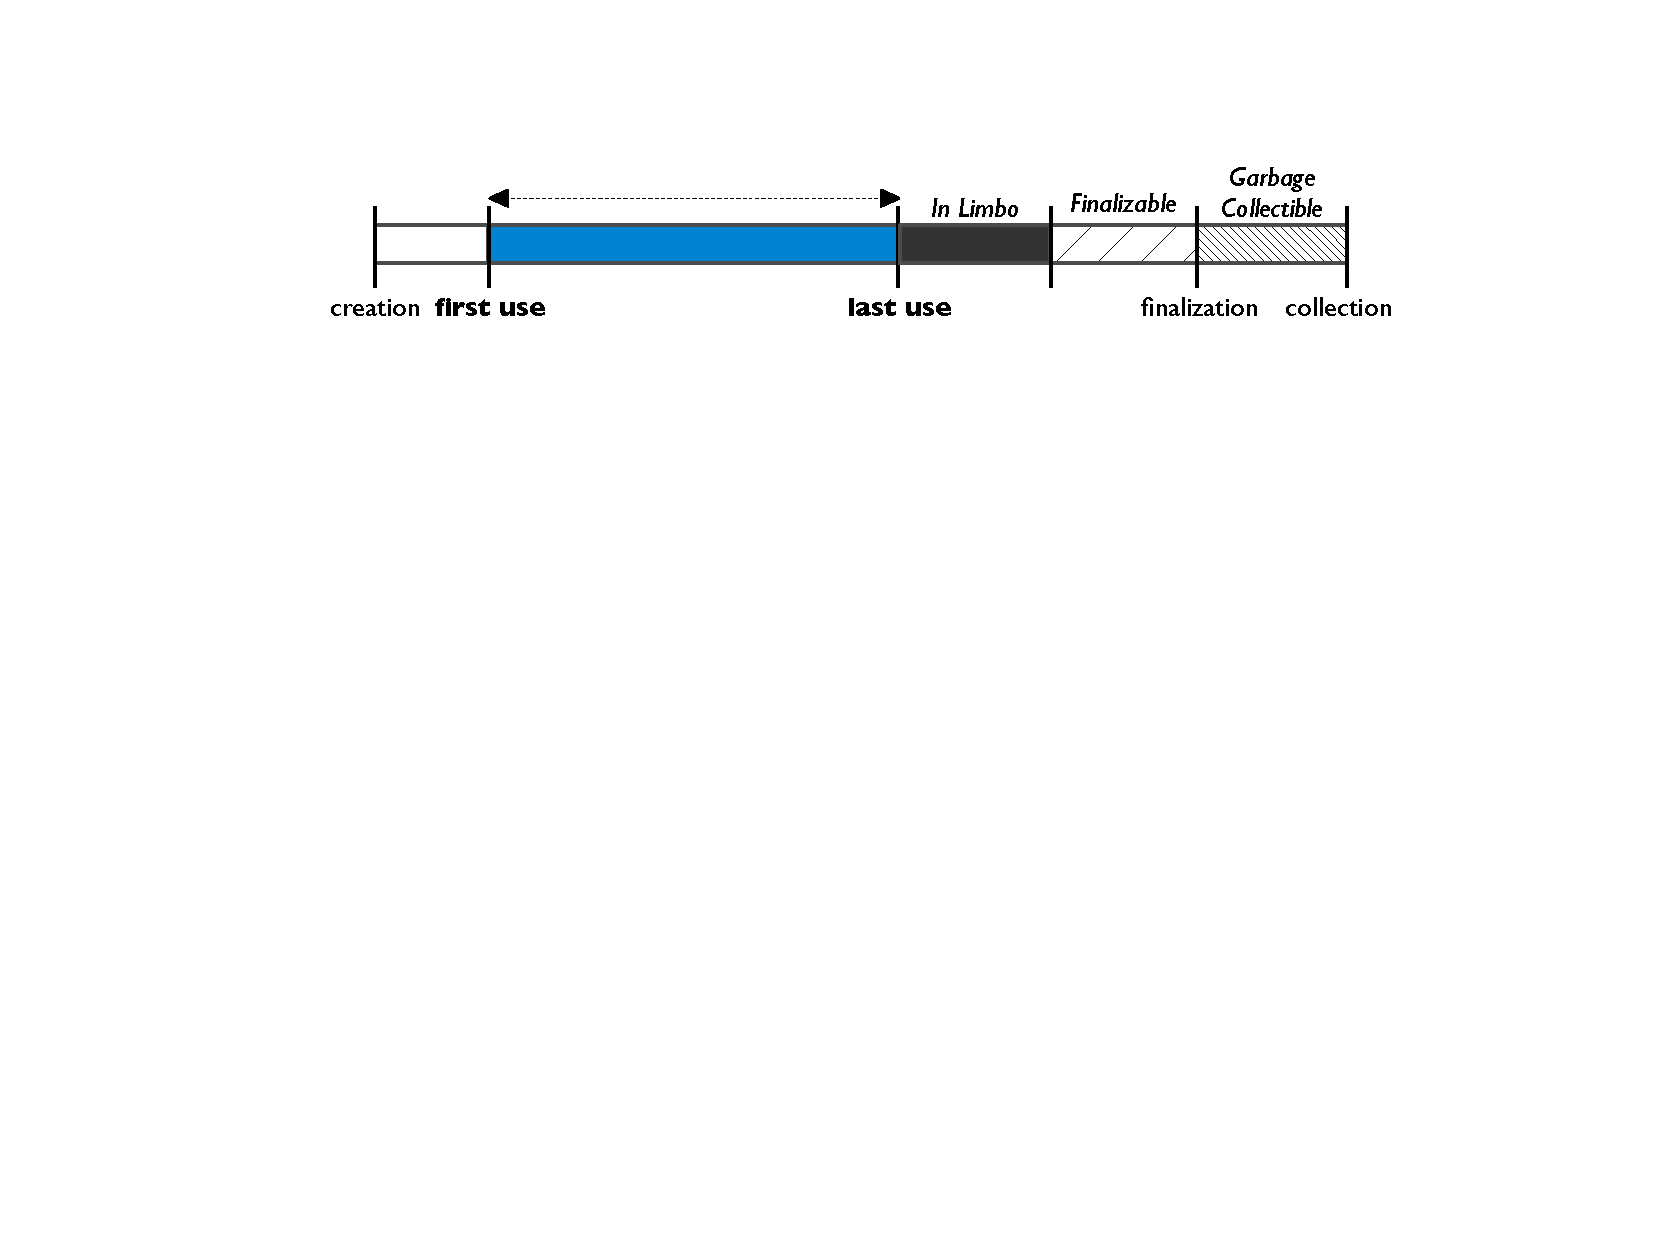
\includegraphics[width=0.95\textwidth]{Figures/lifetime/object-lifecycle}
	}
	\subfigure[A situation where there are long periods between uses of an
	object's data.]{
	\label{fig:typical-lifecycle2}
		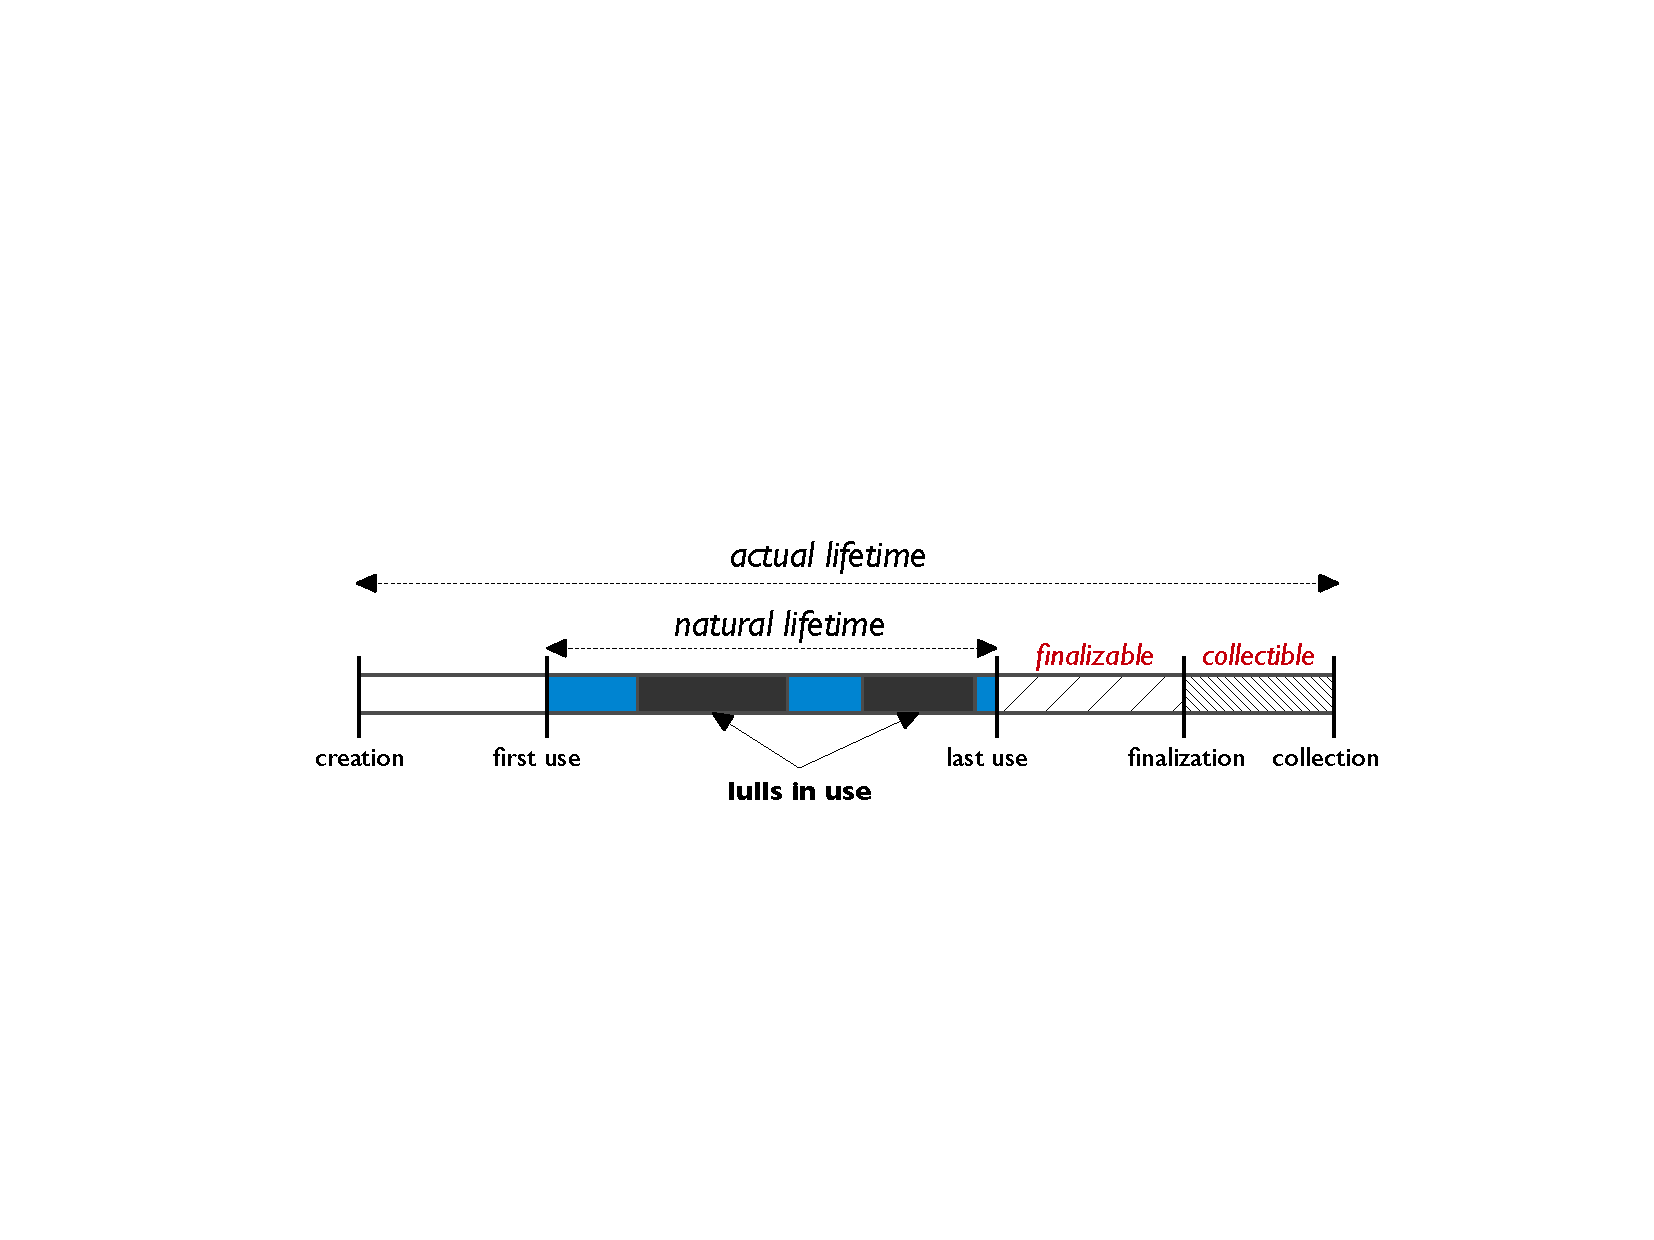
\includegraphics[width=0.95\textwidth]{Figures/lifetme/object-lifecycle-lulls}
	}
	\subfigure[The lifecycle of the data  that is loaded from
	disk three times, and the objects that store it.]{
	\label{fig:typical-lifecycle3}
		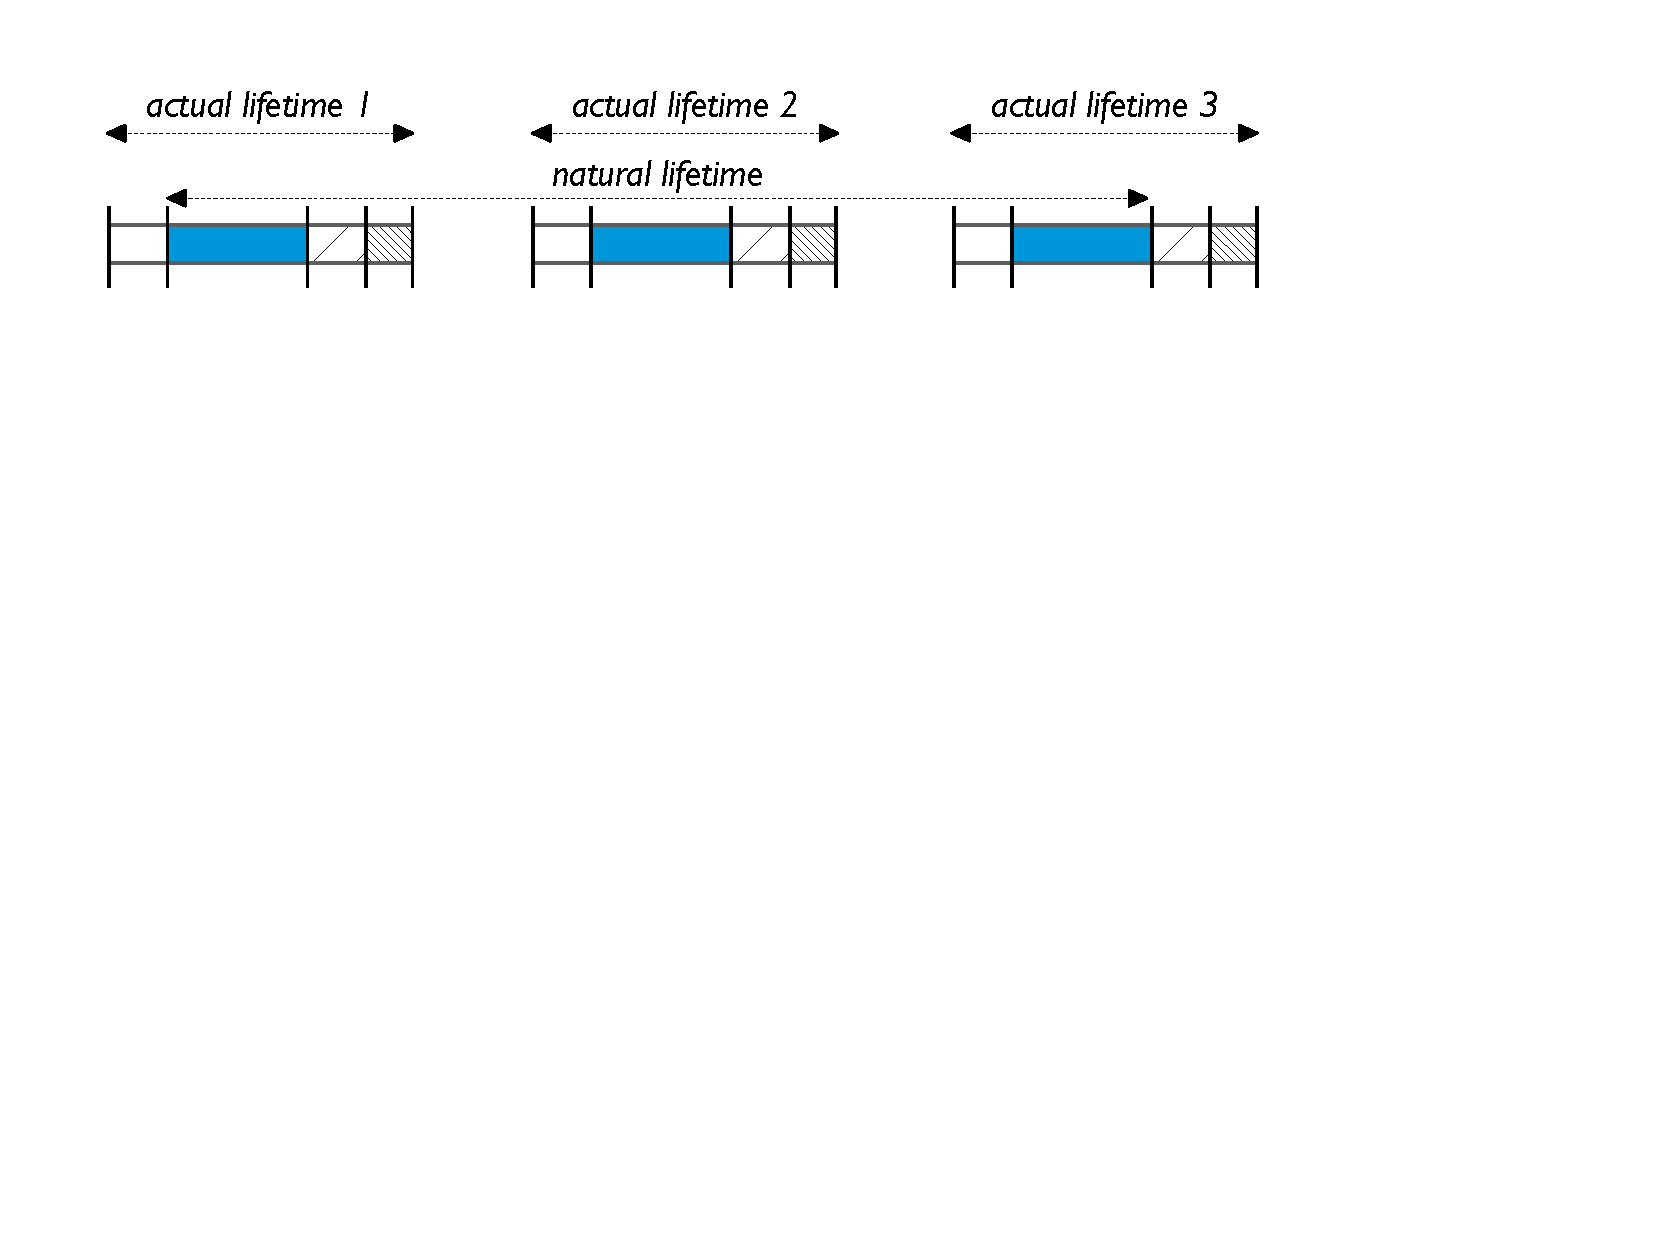
\includegraphics[width=0.9\textwidth]{Figures/object-lifecycle2}
	}
	\caption{Examples of Natural and Actual lifetimes.}
	\label{fig:typical-lifecycle}
\end{figure}
\end{comment}


